\documentclass[aspectratio=169]{beamer}
\geometry{paperwidth=160mm,paperheight=100mm}
\usepackage{beamerthemesidebar}
\usepackage{hyperref}
\usepackage{color}
\usepackage{multimedia}
\usepackage{colortbl}
\usepackage{amsmath}
\usepackage{empheq}
\usepackage{cancel}
\usepackage{amssymb}
\usepackage{amsfonts}
\usepackage{lipsum}
\usepackage{tcolorbox}
\usepackage{tabularx}
\usepackage{caption}
\usepackage{bm}

\setbeamersize{sidebar width right=0pt}
\setbeamertemplate{footline}[frame number]
%
\definecolor{orange}{RGB}{250,167,12}
\definecolor{yellow}{RGB}{246,250,12}
\definecolor{green}{RGB}{128,238,1}
\definecolor{black}{RGB}{0,0,0}
\definecolor{blue}{RGB}{0,0,255}
\definecolor{red}{RGB}{255,0,0}
\definecolor{sepia}{RGB}{94,38,18}
\newcommand{\ve}[1]{{\rm\bf {#1}}}
\newcommand{\q}[1]{\textcolor{blue}{#1}}
\newcommand{\blue}[1]{\textcolor{blue}{#1}}
\newcommand{\sepia}[1]{\textcolor{sepia}{#1}}
\newcommand{\red}[1]{\textcolor{red}{#1}}
\newcommand{\green}[1]{\textcolor{green}{#1}}
\newcommand{\yellow}[1]{\textcolor{yellow}{#1}}
\newcommand{\orange}[1]{\textcolor{orange}{#1}}
\definecolor{burlywood}{RGB}{255,211,155}
\definecolor{chocolate}{RGB}{255,127,36}
\definecolor{tan}{RGB}{210,180,140}
%
\def\onethird{{\textstyle{1\over3}}}
\def\twothirds{{\textstyle{2\over3}}}
\def\fourthirds{{\textstyle{4\over3}}}
\def\onehalf{{\textstyle{1\over2}}}
\def\threehalfs{{\textstyle{3\over2}}}
%
\newcommand{\pd}{\partial}
\newcommand{\aMLT}{\alpha_{\rm MLT}}
\newcommand{\Fconv}{F_{\rm conv}}
\newcommand{\Frad}{F_{\rm rad}}
\newcommand{\Ftot}{F_{\rm tot}}
\newcommand{\Hp}{H_p}
\newcommand{\prad}{p_{\rm rad}}
\newcommand{\pgas}{p_{\rm gas}}
%
\title{Theoretical Astrophysics I: Physics of Sun and Stars\\
Lecture 5: Convection in stars versus convection simulations}
\author{\texorpdfstring{\sepia{Petri K\"{a}pyl\"{a} Ivan Mili\'{c}}\newline\blue{\url{pkapyla, milic@leibniz-kis.de}}}{}}
\institute{Institut f\"ur Sonnenphysik - KIS, Freiburg}
\date{\today}
%
\begin{document}
\frame{\titlepage}

% Convective conundrum: velocity amplitudes in the Sun vs. simulations
% Influence of rotation on convection
% Differential rotation.
% Driving on convection: local or non-local?
% Effects of magnetic fields?
% Induction equation
% Dynamo problem.
% Large-scale and small-scale dynamos.


\section{Convection}
%
\frame{
\frametitle{Convection in the Sun}
\begin{minipage}{0.55\linewidth}
\begin{itemize}
\item Several types of convective flows are conjectured to exist in
  the Sun.
\item Granulation is directly observed. Velocity $u \sim 1$~km/s,
  $\ell \sim 10^3$~km, turnover time $\tau_{\rm c} \sim$ a few
  minutes.
\end{itemize}
\end{minipage}
\begin{minipage}{0.4\linewidth}
\begin{figure}
\includegraphics[width=6cm]{figures/Solar_granulation_DKIST.jpg}
\caption*{Solar granulation from the Daniel K. Inoue Solar Telescope
  (DKIST).}
\end{figure}
\end{minipage}
}
%
\frame{
\frametitle{Convection in the Sun}
\begin{minipage}{0.55\linewidth}
\begin{itemize}
\item Several types of convective flows are conjectured to exist in
  the Sun.
\item Granulation is directly observed. Velocity $u \sim 1$~km/s,
  $\ell \sim 10^3$~km, turnover time $\tau_{\rm c} \sim$ a few
  minutes.
\item Supergranulation is observed using the Doppler effect. Velocity
  $u_{\rm h} \sim 300$~m/s, $u_{\rm v} \sim 40$~m/s, $\ell \sim
  20\ldots 35$~Mm, turnover time $\tau_{\rm c} \sim$ about a day.
\item \blue{Why is the signal so weak near the centre of the disk?}
\end{itemize}
\end{minipage}
\begin{minipage}{0.4\linewidth}
\begin{figure}
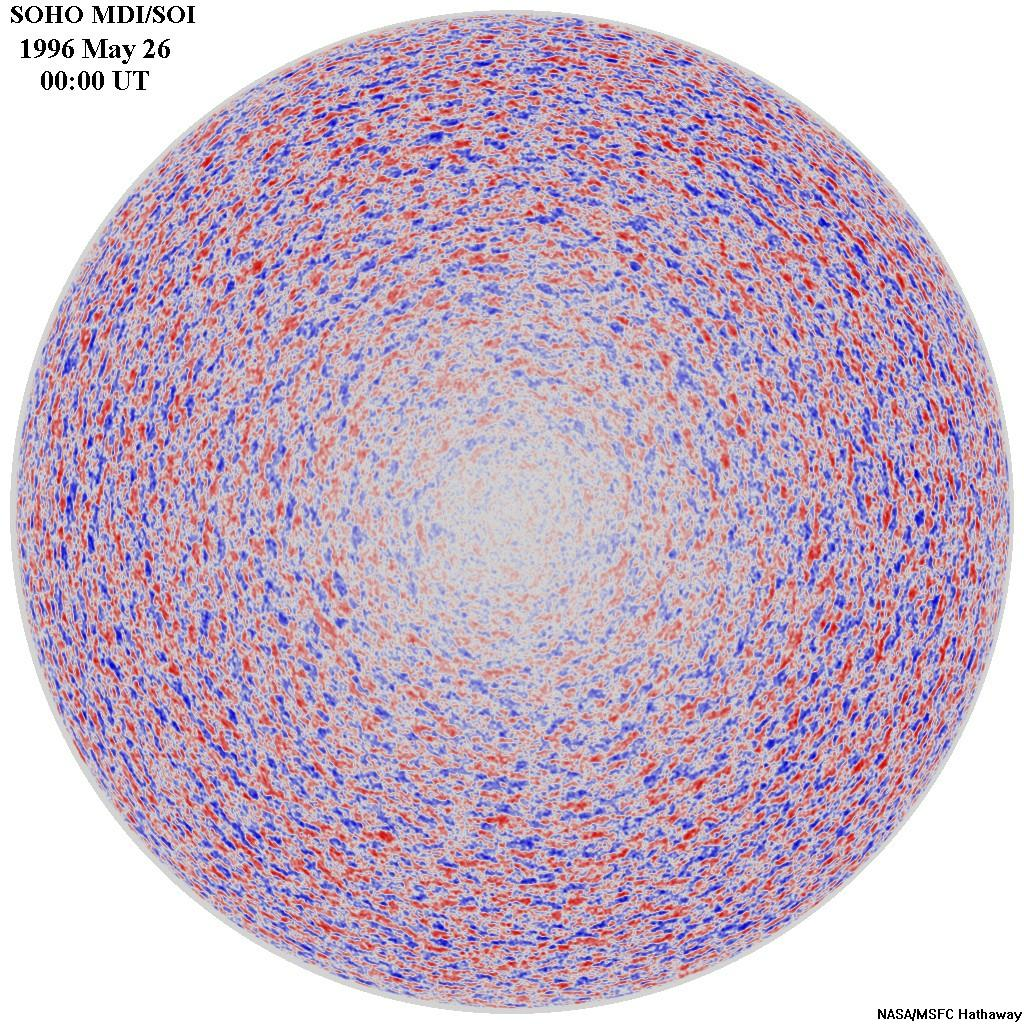
\includegraphics[width=6cm]{figures/Supergranulation.jpg}
\caption*{Solar supergranulation from SOHO MDI.}
\end{figure}
\end{minipage}
}
%
\frame{
\frametitle{Convection in the Sun}
\begin{minipage}{0.55\linewidth}
\begin{itemize}
\item Several types of convective flows are conjectured to exist in
  the Sun.
\item Granulation is directly observed. Velocity $u \sim 1$~km/s,
  $\ell \sim 10^3$~km, turnover time $\tau_{\rm c} \sim$ a few
  minutes.
\item Supergranulation is observed using the Doppler effect. Velocity
  $u_{\rm h} \sim 300$~m/s, $u_{\rm v} \sim 40$~m/s, $\ell \sim
  20\ldots 35$~Mm, turnover time $\tau_{\rm c} \sim$ about a day.
\item Giant cells? $u\sim 10$m/s, $\ell \sim 200$~Mm, $\tau_{\rm
  c}\sim$ a month.
\item \blue{Why would we even expect giant cells?}
\end{itemize}
\end{minipage}
\begin{minipage}{0.4\linewidth}
\begin{figure}
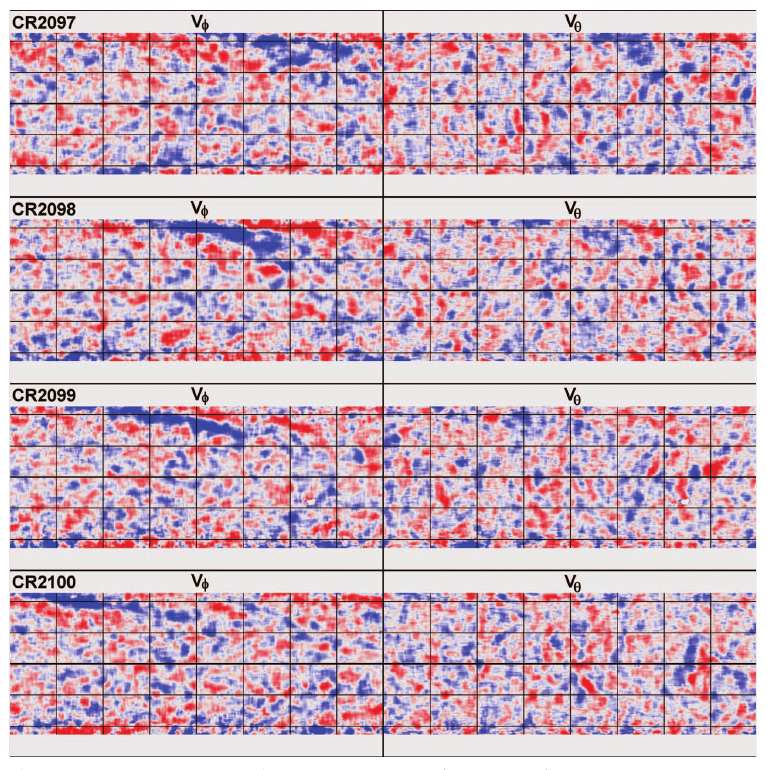
\includegraphics[width=6cm]{figures/Hathaway_Giant_cells.png}
\caption*{Hathaway et al. (2013), Science, 342, 1217.}
\end{figure}
\end{minipage}
}
%
\frame{
\frametitle{Simulations of convection}
\begin{itemize}
\item Simulations solve the equations of (magneto)hydrodynamics in a
  coordinate system most suited to the physical problem:
\end{itemize}

\begin{figure}
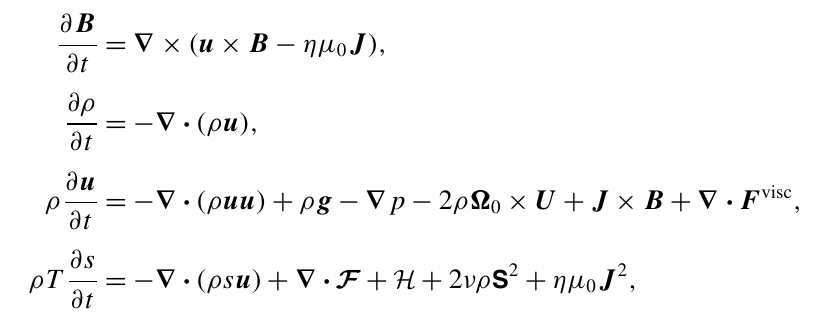
\includegraphics[width=11cm]{figures/MHD_equations.png}
%\caption*{ }
\end{figure}

\begin{itemize}
\item Here, ${\bm F}_{\rm visc} = 2 \nu\rho \bm{\mathsf{S}}$, where
  $\mathsf{S}_{ij} = \onehalf (u_{i,j} + u_{j,i}) - \onethird
  \delta_{ij} \bm\nabla\bm\cdot{\bm u}$ is the traceless
  rate-of-strain tensor, and $\bm{\mathcal{F}}$ contains the radiative
  flux $\bm{\mathcal{F}}_{\rm rad} = -K\bm\nabla T$.
\end{itemize}
}
%
\frame{
\frametitle{Simulations of convection}
\begin{itemize}
\item Simulations solve the equations of (magneto)hydrodynamics in a
  coordinate system most suited to the physical problem:
\end{itemize}

\begin{figure}
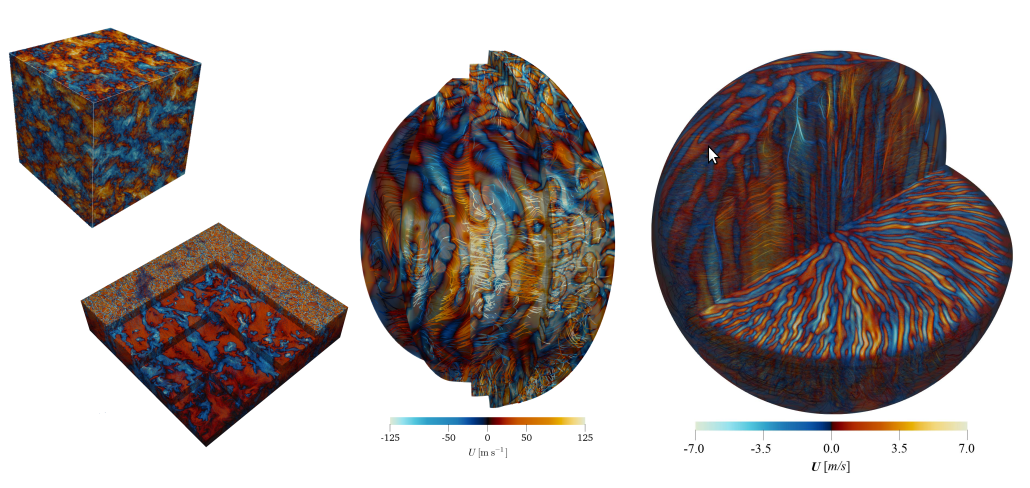
\includegraphics[width=12cm]{figures/Simulation_geometries.png}
\caption*{{\sc Pencil Code}, \href{https://pencil-code.org/}{https://pencil-code.org/}}
\end{figure}
}
%
\frame{
\frametitle{Simulations of solar surface convection}
\begin{figure}
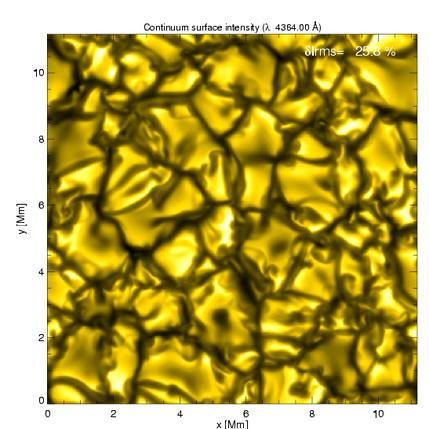
\includegraphics[width=6cm]{figures/Cobold_granulation.jpg}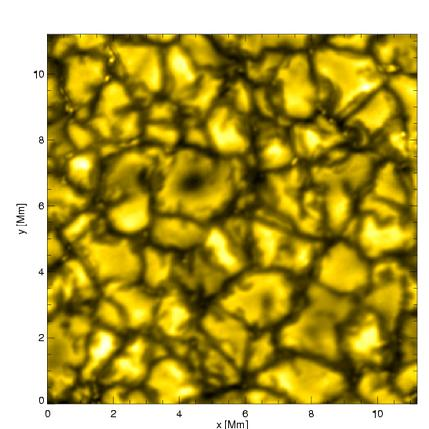
\includegraphics[width=6cm]{figures/SST_granulation.jpg}
\caption*{\blue{Which one is simulation and which on observation?}}
\end{figure}
}
%
%
\frame{
\frametitle{Simulations of solar surface convection}
\begin{figure}
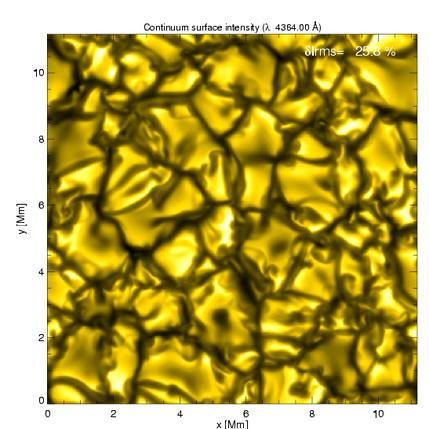
\includegraphics[width=6cm]{figures/Cobold_granulation.jpg}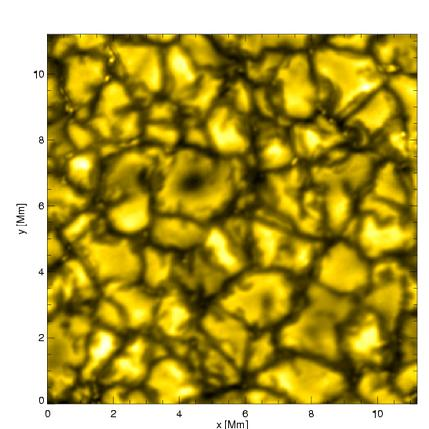
\includegraphics[width=6cm]{figures/SST_granulation.jpg}
\caption*{Left: \blue{Simulated solar surface convection} (credit:
  Matthias Steffen). Right: \blue{Observed granulation} from Swedish
  Solar Telescop (SST) (credit: Mats Carlsson).}
\end{figure}
}
%
%
\frame{
\frametitle{Simulations of global solar convection}
\begin{figure}
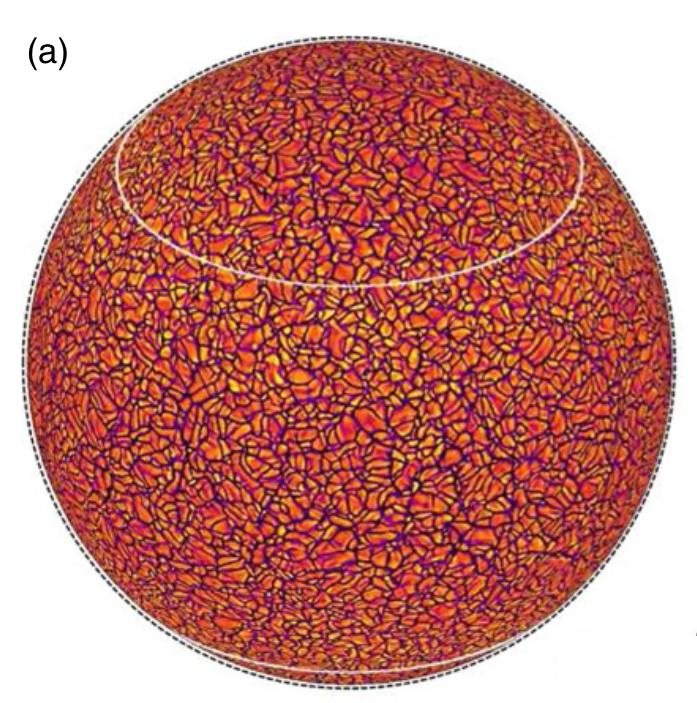
\includegraphics[width=6cm]{figures/Hotta_et_al_2015_granulation.png}\ \ \ 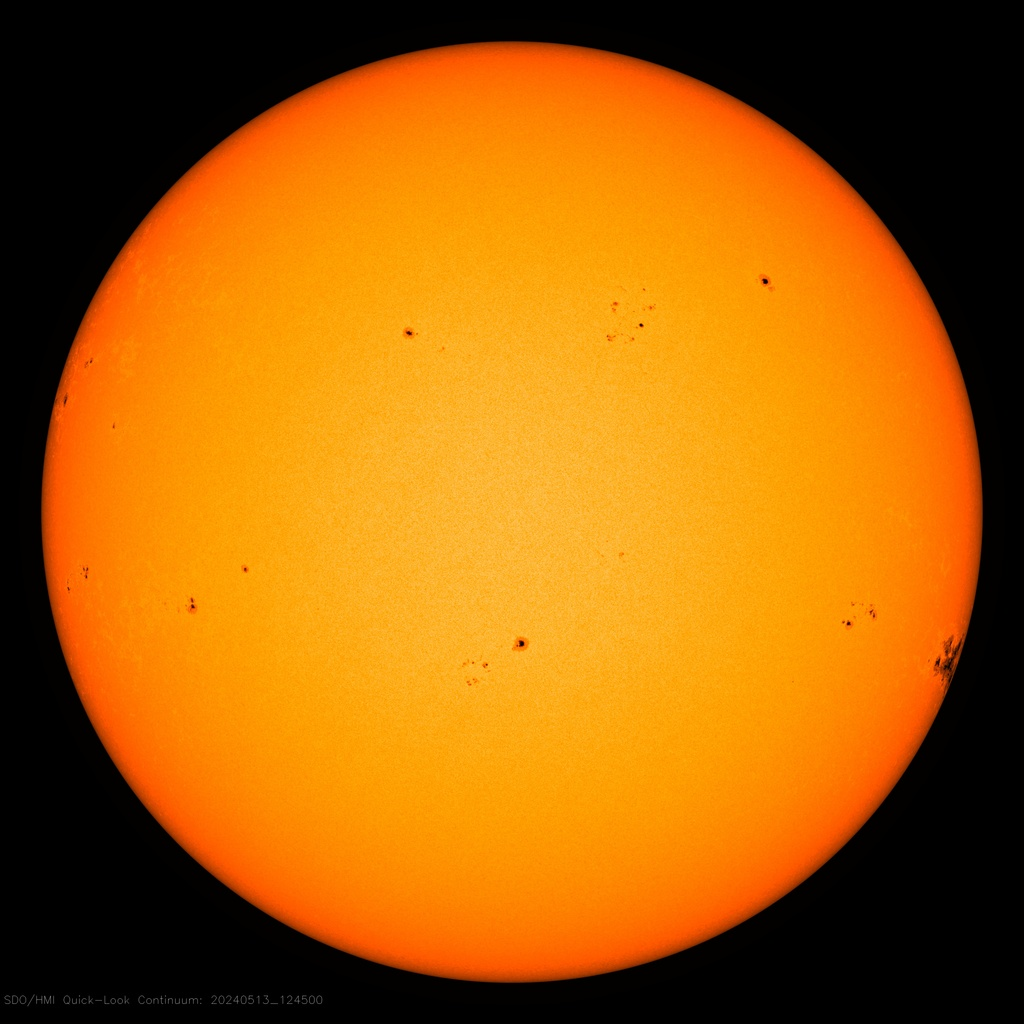
\includegraphics[width=6cm]{figures/HMIIC_13.05.2024.jpg}
\caption*{Left: Radial velocity near the surface of a high-resolution
  global simulation of the Sun (Hotta et al. 2015, Astrophys. J., 798,
  51). Right: HMI Intensitygram from Solar Dynamics Observatory (SDO)
  13.05.2024.}
\end{figure}
}
%
\frame{
\frametitle{Convective conundrum}
\begin{minipage}{0.55\linewidth}
\begin{itemize}
\item Convective velocities observed in the Sun can be used to compute
  the power spectrum of the velocity:
  \begin{equation}
    E_{\rm K} = \onehalf \int E(k)dk,
  \end{equation}
  with $E_{\rm K} = \onehalf {\bm u}^2$ and $E(k) = \sum_k | \hat{\bm
    u}(k) |^2$.
\item While the surface simulations (Stagger) seem to be largely
  compatible with the granulation tracking observations, global
  simulations (ASH) suggest velocities that are much larger.
\item This is one of the manifestations of the ``Convective
  conundrum,'' or the discrepancy between models and reality.
\end{itemize}
\end{minipage}
\hfill
\begin{minipage}{0.4\linewidth}
\begin{figure}
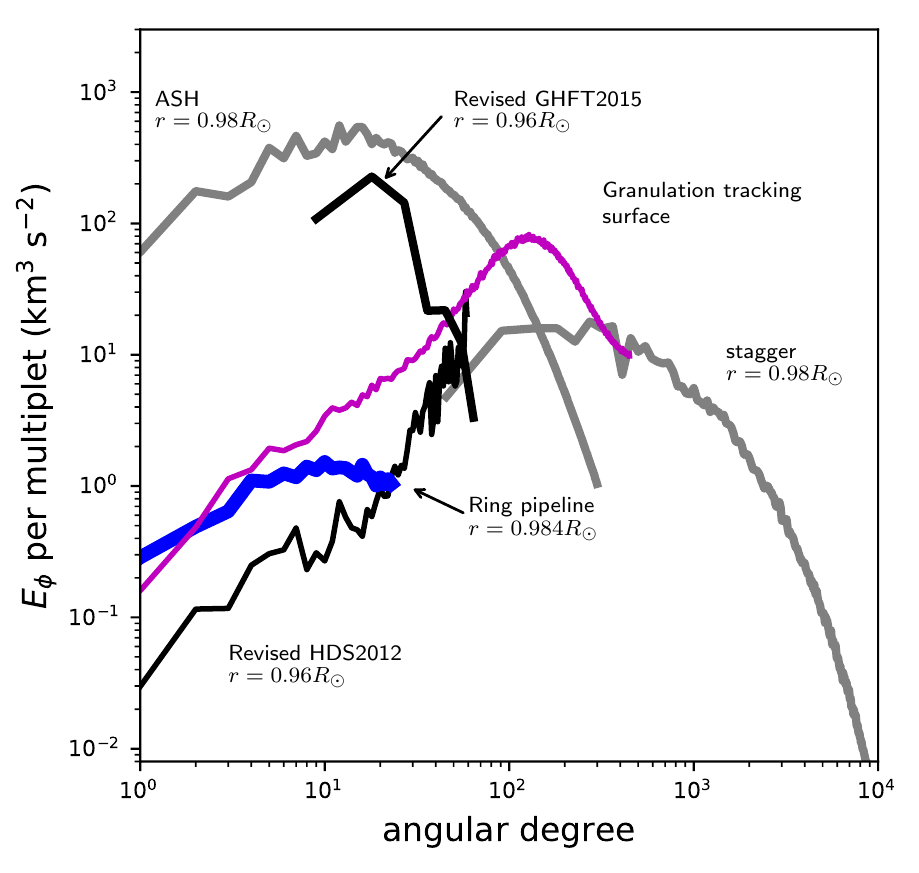
\includegraphics[width=6.5cm]{figures/Proxauf_power_spectrum.png}
\caption*{Proxauf (2021), PhD Thesis (G\"ottingen Univ.)}
\end{figure}
\end{minipage}
}
%
\frame{
\frametitle{Differential rotation}
The Sun rotates \emph{differentially}, i.e., not like a solid body. Here $\Omega = u_\phi/r \sin\theta$.
\begin{minipage}{0.49\linewidth}
\begin{figure}
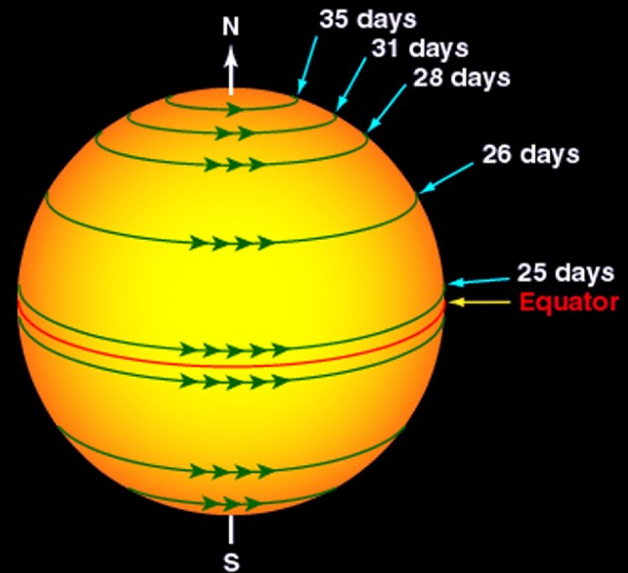
\includegraphics[width=6cm]{figures/solar_DR_surf.png}
\caption*{Source: NASA.}
\end{figure}
\end{minipage}
\hfill
\begin{minipage}{0.5\linewidth}
\begin{figure}
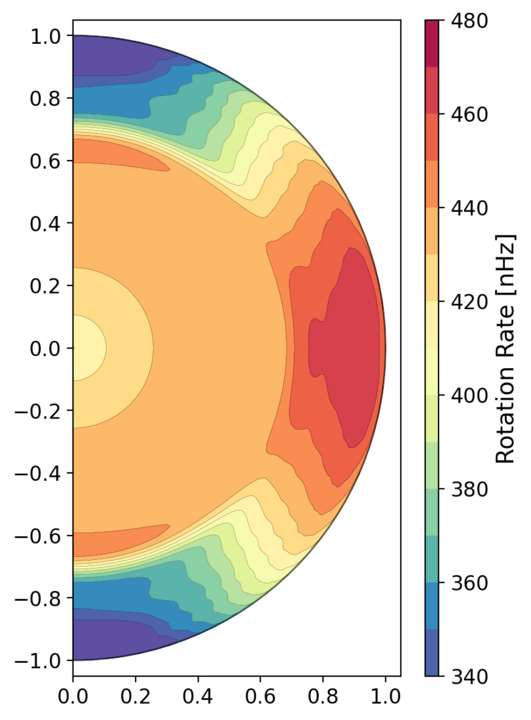
\includegraphics[width=5cm]{figures/solar_DR_int.png}
\caption*{Source: Larson and Schou (2018).}
\end{figure}
\end{minipage}
}
%
%
\frame{
\frametitle{Differential rotation in simulations}
\begin{minipage}{0.44\linewidth}
\begin{itemize}
\item The interaction of convection and the global solar rotation lead
  to differential rotation.
\item Simulations with solar parameters (only luminosity and rotation
  rate as we will see below!) very often yield ``anti-solar''
  differential rotation with fast poles and slow equator.
\item \blue{What simple argument can explain the anti-solar states?}
\end{itemize}
\end{minipage}
\hfill
\begin{minipage}{0.55\linewidth}
\begin{figure}
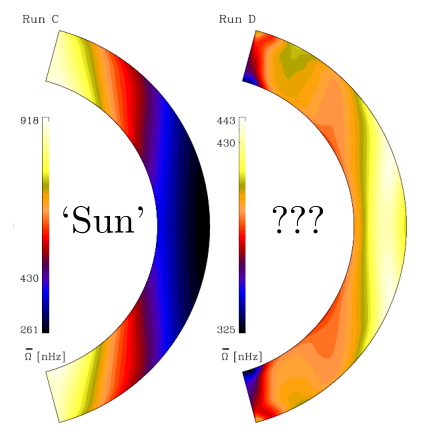
\includegraphics[width=6cm]{figures/DR_KKB14.png}
\caption*{Mean angular velocity $\overline{\Omega} =
  \overline{u}_\phi/r \sin\theta + \Omega_0$. From K\"apyl\"a et
  al. (2014), Astron. Astrophys., 570, 43}
\end{figure}
\end{minipage}
}
%
%
\frame{
\frametitle{Differential rotation in simulations}
\begin{minipage}{0.44\linewidth}
\begin{itemize}
\item Simulations show that the flip fron anti-solar (Regime II) to
  solar-like (Regime I) occurs around ${\rm Ro}_c \sim {\rm Co}^{-1}
  \sim 1$.
\item The Sun appears to be near this transition and simulations tend
  to underestimate ${\rm Co}$.
\end{itemize}
\end{minipage}
\hfill
\begin{minipage}{0.55\linewidth}
\begin{figure}
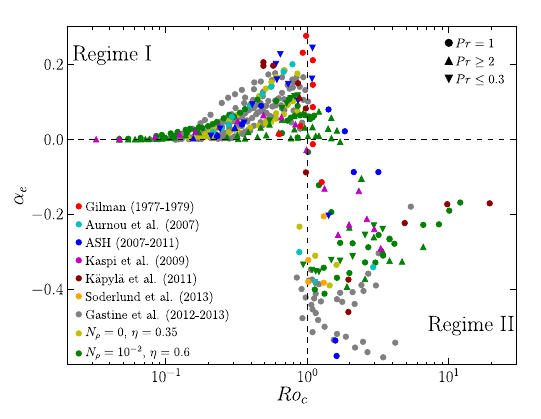
\includegraphics[width=8cm]{figures/DR_Gastine_2014.png}
\caption*{Source: Gastine et al. (2014), MNRAS, 438, L76.}
\end{figure}
\end{minipage}
}
%
%
\frame{
\frametitle{Convection and rotation}
\begin{minipage}{0.55\linewidth}
\begin{itemize}
\item As we discussed in the last tutorial, the order of magnitude of
  the convective velocity and length scale are
  \begin{equation}
    u \sim \left(\frac{\Ftot}{\rho} \right)^{1/3} \equiv u_\star,\ \mbox{and} \ \ell \sim H_p,
  \end{equation}
  where $\Ftot = \frac{L}{4\pi r^2}$ and $\rho$ is a reference
  density.
\item We also saw on the previous lecture that according to the mixing
  length theory the Coriolis number
  \begin{equation}
    {\rm Co} = \frac{2\Omega_\odot \ell}{u},
  \end{equation}
  varies between $10^{-3}$ near the surface and around $10$ at the
  base of the convection zone.
\end{itemize}
\end{minipage}
\hfill
\begin{minipage}{0.4\linewidth}
\begin{figure}
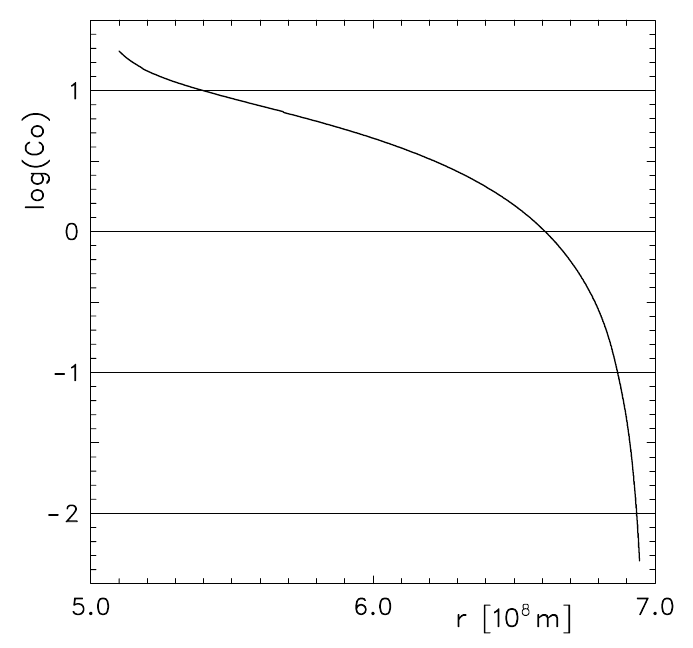
\includegraphics[width=6cm]{figures/MLT-Sun_Co.png}
\caption*{K\"apyl\"a et al. (2005), Astron. Astrophys., 438, 403.}
\end{figure}
\end{minipage}
}
%
\frame{
\frametitle{Convection and rotation}
\begin{minipage}{0.49\linewidth}
\begin{itemize}
\item When rotation is sufficiently rapid, the rotating mixing length
  theory (e.g. Stevenson, 1979, Geophys. Astrophys. Fluid Dyn., 12,
  139) predicts that the convective velocity changes and is
  \begin{equation}
    u \sim \left(\frac{\Ftot}{\rho} \right)^{1/3} {\rm Co}^{-1/6} = u_\star {\rm Co}^{-1/6},
  \end{equation}
\item \blue{Where is the Sun in this diagram?}
\end{itemize}
\end{minipage}
\hfill
\begin{minipage}{0.5\linewidth}
\begin{figure}
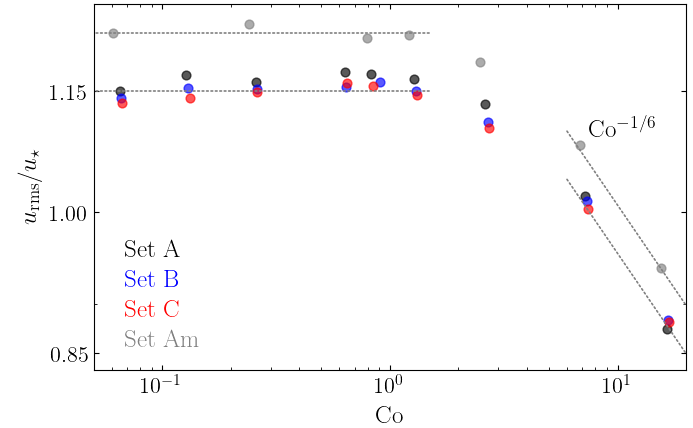
\includegraphics[width=7cm]{figures/plot_urms_Co.png}
\caption*{Convective velocity divided by $u_\star$ from several sets
  of simulations. From K\"apyl\"a (2024), Astron. Astrophys., 683,
  221.}
\end{figure}
\end{minipage}
}
%
\frame{
\frametitle{Convection and rotation}
\begin{minipage}{0.49\linewidth}
\begin{itemize}
\item When rotation is sufficiently rapid, the rotating mixing length
  theory (e.g. Stevenson, 1979, Geophys. Astrophys. Fluid Dyn., 12,
  139) predicts that the convective velocity changes and is
  \begin{equation}
    u \sim \left(\frac{\Ftot}{\rho} \right)^{1/3} {\rm Co}^{-1/6} = u_\star {\rm Co}^{-1/6},
  \end{equation}
\item \blue{Where is the Sun in this diagram?}
\end{itemize}
\end{minipage}
\hfill
\begin{minipage}{0.5\linewidth}
\begin{figure}
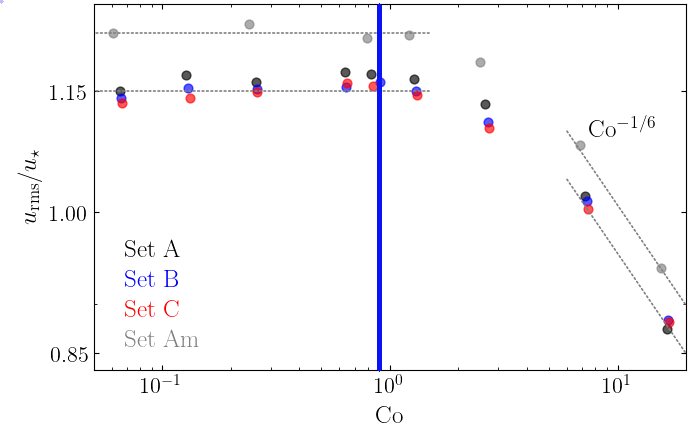
\includegraphics[width=7cm]{figures/plot_urms_Co_sun.png}
\caption*{Convective velocity divided by $u_\star$ from several sets
  of simulations. From K\"apyl\"a (2024), Astron. Astrophys., 683,
  221.}
\end{figure}
\end{minipage}
}
%
%
\frame{
\frametitle{Convection and rotation}
\begin{minipage}{0.49\linewidth}
\begin{itemize}
\item The convective length scale also changes
  \begin{equation}
    \ell \sim H_p {\rm Co}^{-1/2}.
  \end{equation}
\item It appears that convection in the deep parts of solar convection
  zone are less rotationally constrained than previously thought.
\end{itemize}
\end{minipage}
\hfill
\begin{minipage}{0.5\linewidth}
\begin{figure}
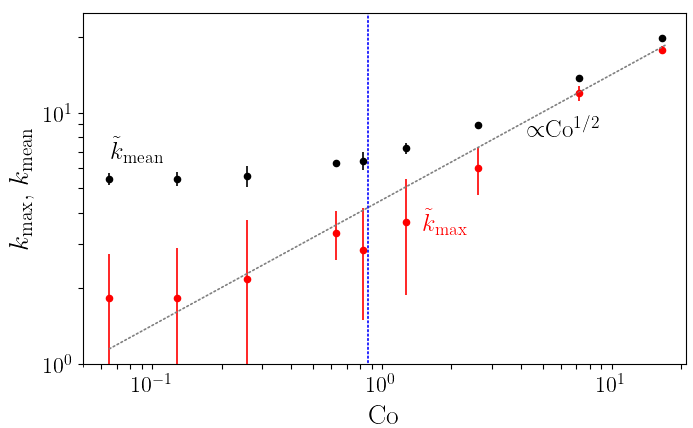
\includegraphics[width=7cm]{figures/plot_length_iau.png}
\caption*{Two measures of the scale ($k = 2\pi/\ell$) of convective
  structures in simulations as functions of ${\rm Co}$. From
  K\"apyl\"a (2023), arXiv:2311.09082.}
\end{figure}
\end{minipage}
}
%
%
\frame{
\frametitle{Convection and rotation}
\begin{minipage}{0.49\linewidth}
\begin{itemize}
\item The convective length scale also changes
  \begin{equation}
    \ell \sim H_p {\rm Co}^{-1/2}.
  \end{equation}
\item It appears that convection in the deep parts of solar convection
  zone are less rotationally constrained than previously thought.
\item There is a catch, however, and we will come back to that later.
\end{itemize}
\end{minipage}
\hfill
\begin{minipage}{0.5\linewidth}
\begin{figure}
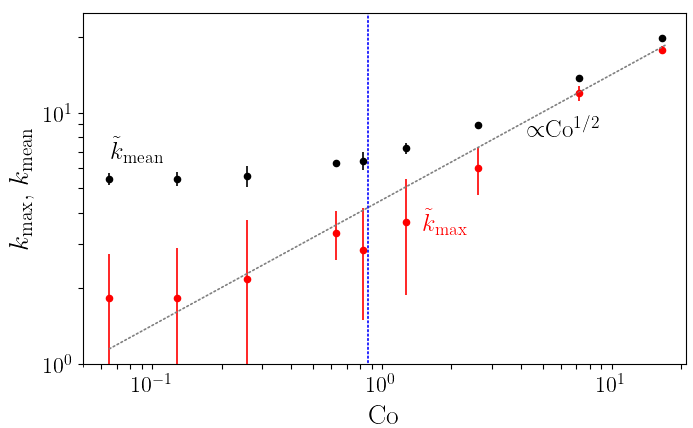
\includegraphics[width=7cm]{figures/plot_length_iau.png}
\caption*{Two measures of the scale ($k = 2\pi/\ell$) of convective
  structures in simulations as functions of ${\rm Co}$. From
  K\"apyl\"a (2023), arXiv:2311.09082.}
\end{figure}
\end{minipage}
}
%
\frame{
\frametitle{Why do simulations struggle to reproduce the Sun?}

\begin{itemize}
\item \blue{Any ideas?}
\end{itemize}
}
%
\frame{
\frametitle{Why do simulations struggle to reproduce the Sun?}
\begin{itemize}
\item The equations of magnetohydrodynamics can be written in a
  dimensionless form where a number of dimensionless quantities
  uniquely defining the system appear (tutorial).
\end{itemize}

\begin{figure}
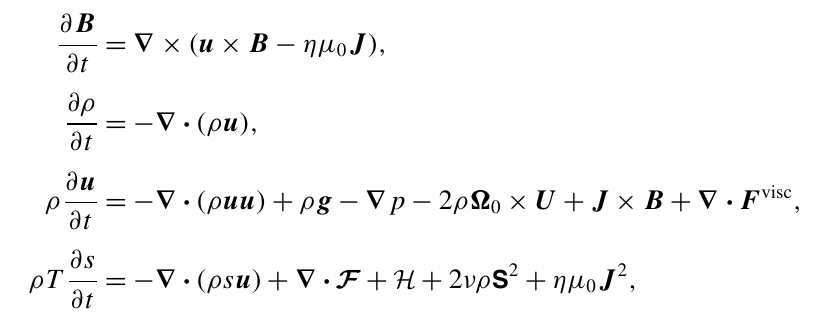
\includegraphics[width=11cm]{figures/MHD_equations.png}
%\caption*{ }
\end{figure}
}
%
%
\frame{
\frametitle{Why do simulations struggle to reproduce the Sun?}

\begin{itemize}
\item The equations of magnetohydrodynamics can be written in a
  dimensionless form where a number of dimensionless quantities
  uniquely defining the system appear.
\item These include the Prandtl numbers, the Rayleigh number, and the
  Taylor number:
  \begin{equation}
    {\rm Pr} = \frac{\nu}{\chi},\ \ {\rm Pr}_{\rm M} = \frac{\nu}{\eta}, \ \ {\rm Ra} = \frac{gd^4}{\nu\chi} \left( -\frac{1}{c_p} \frac{ds}{dr}\right), \ \ {\rm Ta} = \frac{4\Omega^2d^4}{\nu^2},
  \end{equation}
  where $\nu$ is the kinematic viscosity, $\eta$ is the magnetic
  diffusivity, and $\chi = K_{\rm rad}/c_p \rho$ is the radiative
  diffusivity.
\item We can also estimate the relative magnitudes of different terms
  in the equations by OOM (order of magnitude) analysis. These give an
  additional set of (diagnostic) numbers (Reynolds, P\'eclet, Coriolis):
  \begin{equation}
    {\rm Re} = \frac{ud}{\nu},\ \ {\rm Re}_{\rm M} = \frac{ud}{\eta},\ \ {\rm Pe} = \frac{ud}{\chi}, \ \ {\rm Co} = \frac{2\Omega d}{u}.
  \end{equation}
  \item We need to compare these quantities in the simulations to
    those in stars.
\end{itemize}
}
%
%
\frame{
\frametitle{Why do simulations struggle to reproduce the Sun?}

\begin{itemize}
  \item Typically these numbers in stars are either $\gg 1$ or $\ll 1$.
  \item Simulations are limited by available computational resources
    and can for most parameters do only modest values.
\end{itemize}

\begin{figure}
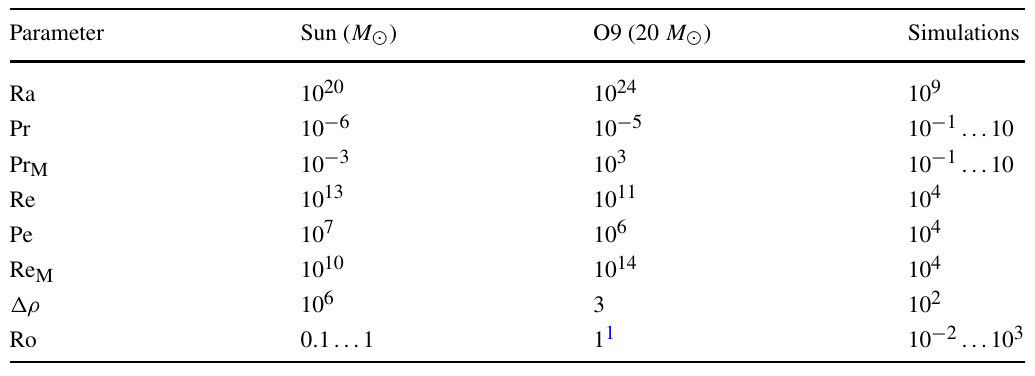
\includegraphics[width=10cm]{figures/Params_Ketal_2023.png}
\caption*{Some dimensionless parameters in the Sun and in a
  $20M_\odot$ O9 star in comparison to typical simulations. From
  K\"apyl\"a et al. (2023), Space Science Rev., 219, 58.}
\end{figure}
Only the Rossby number (${\rm Co}^{-1}$) can be reproduced!
}
%
%
\frame{
\frametitle{Why do simulations struggle to capture the Sun?}

\begin{itemize}
\item More precisely, another Coriolis number can be defined as
  \begin{equation}
    {\rm Co}_\star = \frac{2\Omega H_p}{u_\star},
  \end{equation}
  that does not depend on any actual velocity or length scale. It
  turns out that
  \begin{equation}
    {\rm Co}_\star = ({\rm Ra}_{\rm F}^\star)^{-1/3},\ \ \mbox{where}\ \ {\rm Ra}_{\rm F}^\star = \frac{{\rm Ra}_{\rm F}}{{\rm Pr}^2{\rm Ta}^{3/2}}.
  \end{equation}
  \item The catch mentioned earlier is that it is not enough to
    reproduce \emph{one} of the system parameters if all the other
    ones are (too much) off.
  \item We will come back to this in the tutorial...
\end{itemize}
}
%
%
\frame{
\frametitle{Non-canonical models of convection}

\begin{itemize}
\item \red{Heating from the bottom} or \blue{cooling at the top}?
\item Instead of $\nabla-\nabla_{\rm a} >0$ everywhere (as in mixing
  length theory), perhaps the lower part of the convection zone is
  \emph{stably stratified}? This happens in the case of surface
  cooling driven convection.
\end{itemize}
\begin{figure}
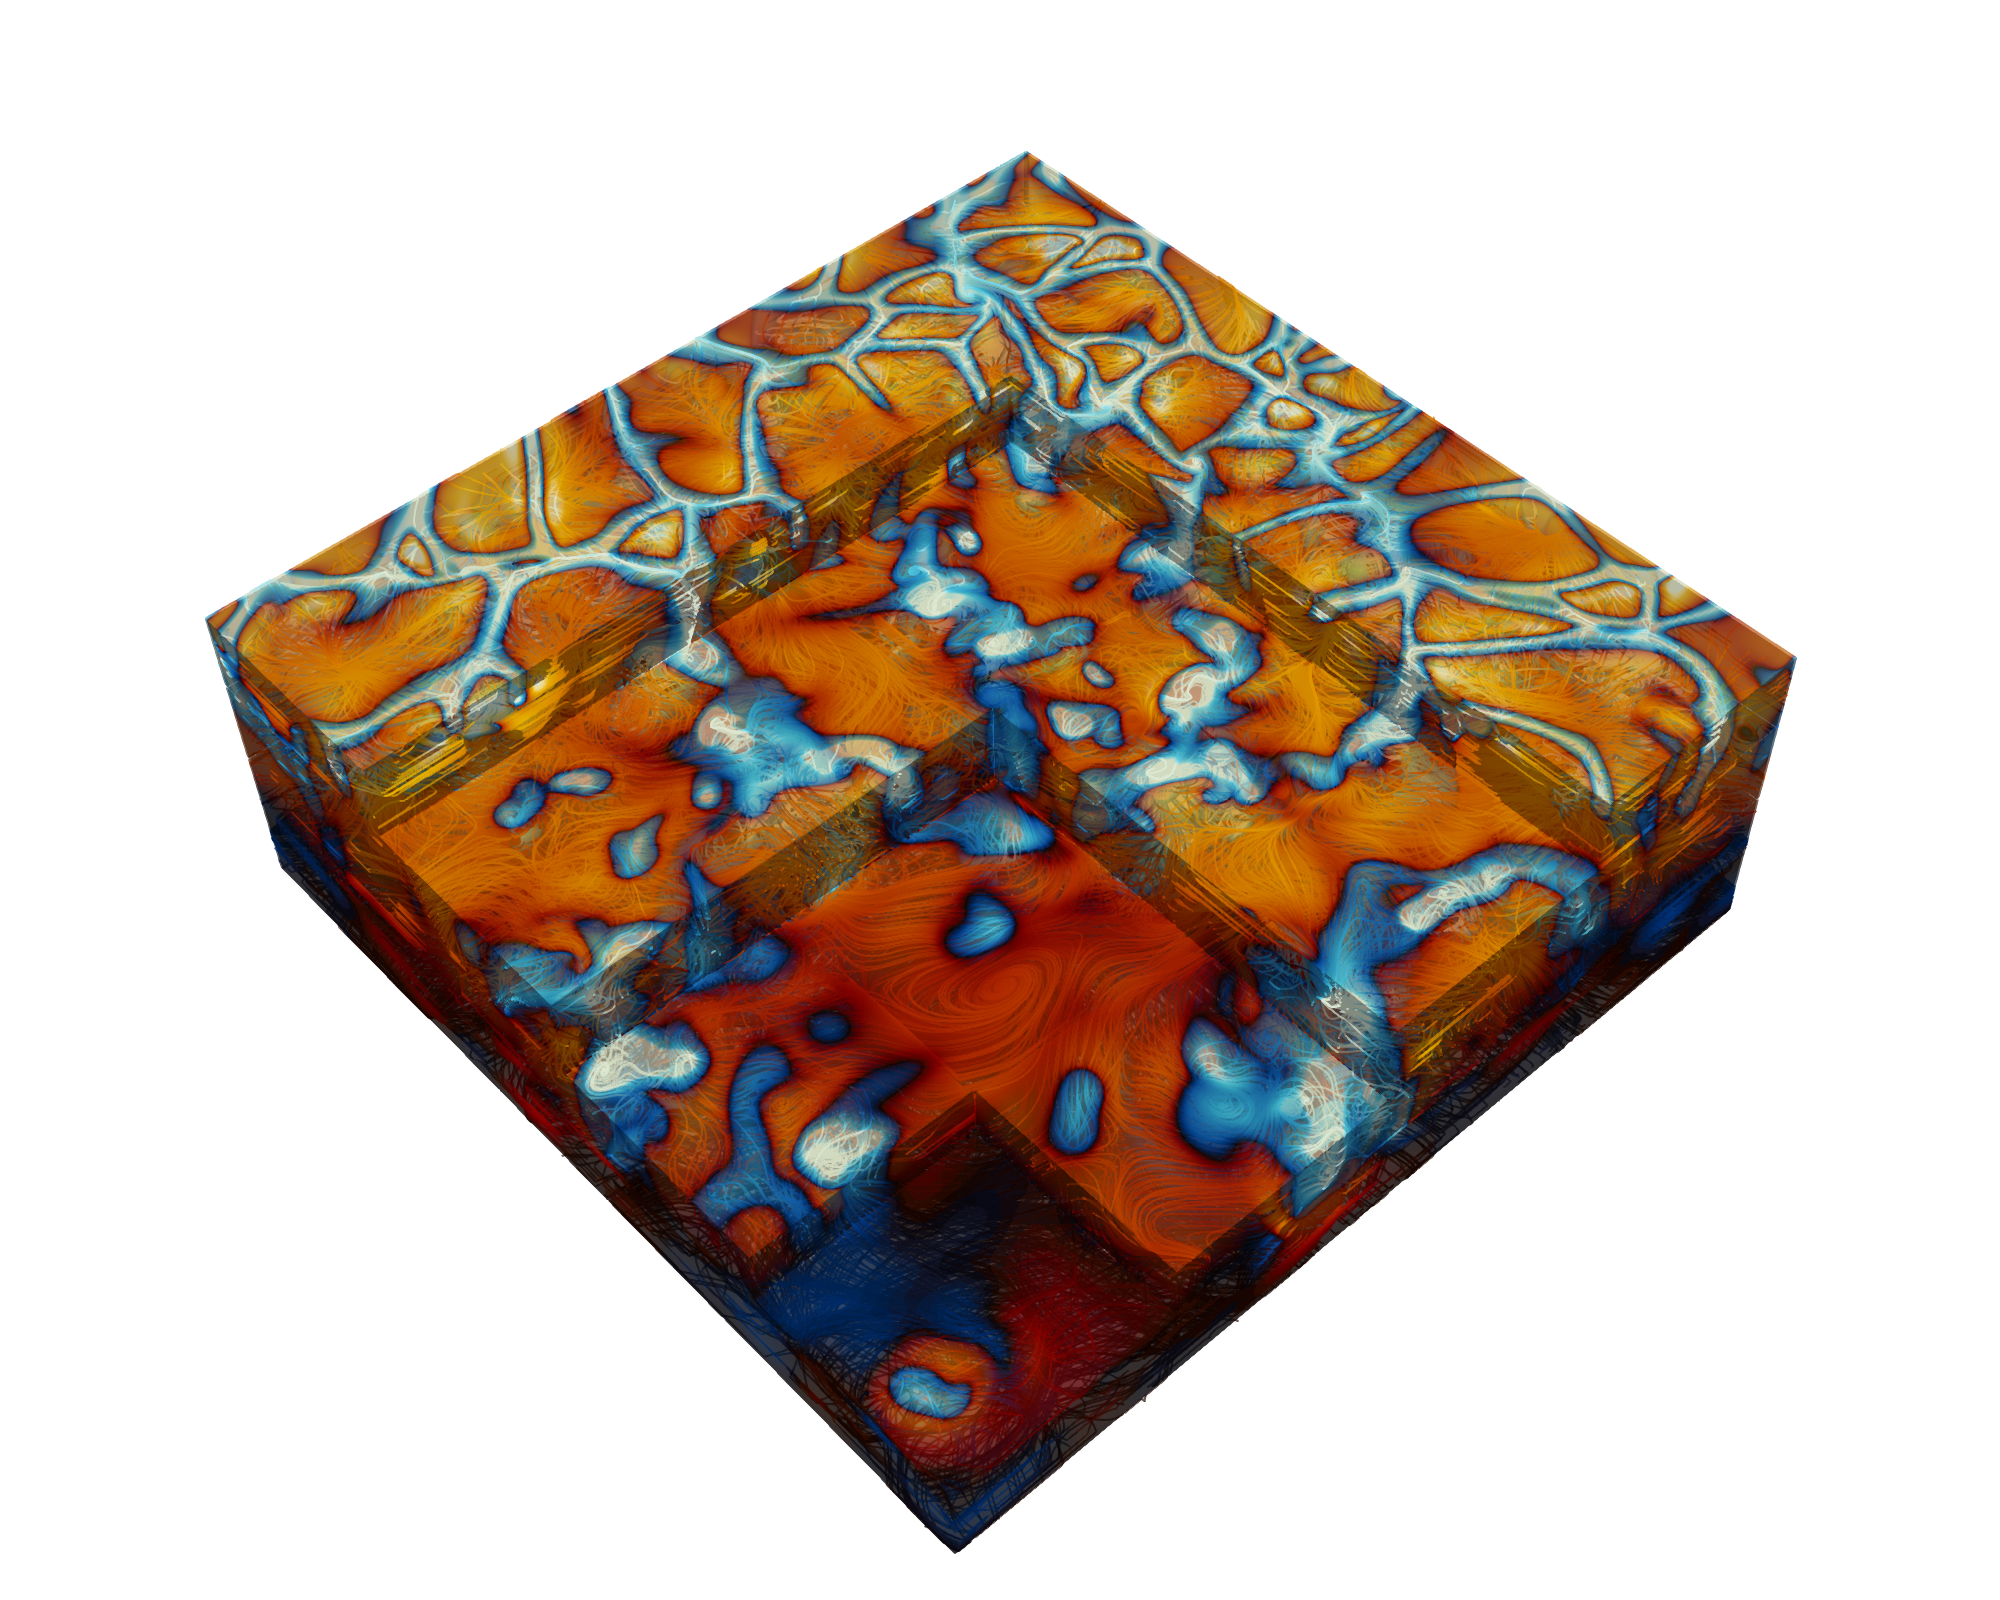
\includegraphics[width=6cm]{figures/conv-norot.png}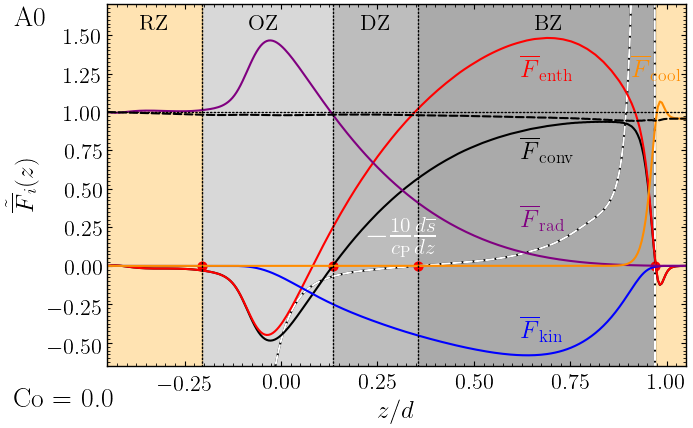
\includegraphics[width=7cm]{figures/plot_fluxes_Om00_288.png}
\caption*{Left: snapshot of the velocity. Right: Energy fluxes and the
  negative of the entropy gradient. Grey areas mixed by convection!}
\end{figure}
}
%
%
\frame{
\frametitle{Why should we care?}
\begin{itemize}
\item The evolution of the magnetic field is governed by
  \begin{equation}
    \frac{\pd {\bm B}}{\pd t} = \bm\nabla \times ({\bm u} \times {\bm B} - \eta \mu_0 {\bm J}),
  \end{equation}
  where ${\bm J} = \mu_0^{-1} \bm\nabla \times {\bm B}$ is the current
  density.
\item If ${\bm u} = 0$, the induction equation reduces to a
  \emph{diffusion equation}:
  \begin{equation}
    \frac{\pd {\bm B}}{\pd t} = \eta \nabla^2{\bm B}.
  \end{equation}
\item \blue{Why is this relevant?}
\end{itemize}
}
%
%
\frame{
\frametitle{Why should we care?}
\begin{itemize}
\item The evolution of the magnetic field is governed by
  \begin{equation}
    \frac{\pd {\bm B}}{\pd t} = \bm\nabla \times ({\bm u} \times {\bm B} - \eta \mu_0 {\bm J}),
  \end{equation}
  where ${\bm J} = \mu_0^{-1} \bm\nabla \times {\bm B}$ is the current
  density.
\item If ${\bm u} = 0$, the induction equation reduces to a
  \emph{diffusion equation}:
  \begin{equation}
    \frac{\pd {\bm B}}{\pd t} = \eta \nabla^2{\bm B}.
  \end{equation}
\item \blue{Why is this relevant?}
\item The field cannot be generated without flows. To understand the
  generation of, e.g., the solar magnetic field, we must now the
  velocity field. \emph{Study of magnetic phenomena is by far the
  most interesting branch of solar physics!}
\end{itemize}
}
%
%% \frame{
%% \frametitle{Large-scale dynamo}

%% \begin{itemize}
%% \item BLAA
%% \end{itemize}
%% }
%% %
%% \frame{
%% \frametitle{Small-scale dynamo}

%% \begin{itemize}
%% \item BLAA
%% \end{itemize}
%% }
%% %
%% \frame{
%% \frametitle{Do all stars have magnetic cycles?}

%% \begin{itemize}
%% \item BLAA
%% \end{itemize}
%% }
%% %
%% %
%% \frame{
%% \frametitle{Rotation-activity correlation}

%% \begin{itemize}
%% \item BLAA
%% \end{itemize}
%% }
%% %
%

\end{document}



